\documentclass[11pt]{report}

\usepackage{array}
\usepackage{graphicx}
\graphicspath{ {./images/} }
\newenvironment{conditions}
  {\par\vspace{\abovedisplayskip}\noindent\begin{tabular}{>{$}l<{$} @{${}={}$} l}}
  {\end{tabular}\par\vspace{\belowdisplayskip}}
\usepackage{fancyhdr}
\usepackage{subfigure}
\usepackage{multirow}
\usepackage{array}
\newcolumntype{P}[1]{>{\centering\arraybackslash}p{#1}}
\usepackage{longtable}
\usepackage{caption}

\usepackage{titlesec}
\setcounter{secnumdepth}{4}
\titleformat{\paragraph}
{\normalfont\normalsize\bfseries}{\theparagraph}{1em}{}
\titlespacing*{\paragraph}
{0pt}{3.25ex plus 1ex minus .2ex}{1.5ex plus .2ex}

\title{Computer science project report}
\author{Lucian James}

\pagestyle{fancy}
\fancyhf{}
\rhead{Centre no 36538}
\lhead{Lucian James - Photogrammetry data cleaner}
\rfoot{Page \thepage}

\begin{document}
\maketitle
\tableofcontents
\thispagestyle{fancy}


\chapter{Analysis}
\thispagestyle{fancy}
% outline - explain the task
\section{Outline} % not much detail
Photogrammetry is a process where a series of overlapping images are analysed to extract 3 dimensional data about the subjects of the images, this data can then be used to produce 3D models which can be used in games and CGI for movies, or 3D printed to produce a replica.
This project aims to produce a piece of software which can be used to process videos for use in photogrammetry software, with a focus on ensuring ease of use with popular open source options.\\\\
The general process of photogrammetry involves taking a series of individual images of the object.
The issue with this is that taking a picture, moving the camera around the object, and repeating can be very time consuming.
Taking a video of the object is much easier, as one can simply walk around the object with the camera pointed at it.\\\\
The problem of needing individual images become especially difficult when doing drone-based photogrammetry, for similar reasons to those described above.

\section{Identification of all stakeholders}
% a client is a stakeholder, but end users are also stakeholders. ANYONE WITH AN INTEREST IN THE PROJECT OR THE OUTCOMES OF THE PROJECT
% interview with stakeholders, get exact details.

\subsection{Stakeholders}
The client for this project is Mr.Parr, one of my computer science and IT teachers.\\\\
The end users of this project include myself, Mr.Parr, and potentially some people on the internet who do photogrammetry, as there are some posts on the internet where individuals have complained about existing solutions, so it is likely that they would be interested in my alternative (see section \ref{research}).
\subsection{Stakeholder descriptions}
Myself: i occasionally do 3D modelling in my spare time, sometimes involving photogrammetry.\\\\
Mr.Parr: Wannabe game dev or something.\\\\
Internet people: This group of people who may be interested in using this software is very broad, but generally it is more likely that they will not be professionals and will make use of open source software more often that proprietary software, this is due to the fact that my existing (small, but existing) youtube audience is compromised entirely of blender users. I will be showcasing this software on my youtube channel mainly, but i may showcase it on other websites
\subsection{How stakeholders will make use of proposed solution}
I would use this software occasionally for personal photogrammetry projects. It would be appropriate for my personal projects as i would prefer to use an easy and efficient piece of software to convert captured videos into usable image data.\\\\
Mr.Parr has described why he needs this software produced: 
\begin{quote}
``I would like to be able to use my phone and drone to use the video capture option instead of taking many still images. As the delay between pressing the button and capturing the image can cause issues. It means I could focus on flying/walking/moving smoothly and extract image later''
\end{quote}
Essentially Mr.Parr will be using this software primarily for hobby purposes, he will use this software to speed up the process of creating 3D models from videos, saving his precious time to focus on the more important aspects of his projects.\\\\
Users on the internet may use this project for photogrammetry projects where they have or would prefer to capture video footage as the source data. My software could be more appropriate than existing methods and this is evidenced by the fact i have seen individuals complain about the current existing solutions and methods for performing the task of converting video into image data usable for photogrammetry.

\subsection{Why the proposed solution is suitable for the stakeholders needs}
The proposed solution will be well suited to my needs as the development will be guided partly by my personal preferences when there is no information given by the client for the particular part of the program being developed.
A lot of the features of the program are suggestions to the client from myself, based on what i would i believe is required to create the most optimal image dataset from a given video for the process of photogrammetry.\\\\
The proposed solution will be suitable for the needs of the client as I intend on writing the program in such a way that it performs all the basic tasks he originally asked for, as well as more advanced functions that I believe could be very useful. The basic requirements outlined by the client can be achieved reasonably easily (see section \ref{feat}), and I am sure that I will meet these requirements reasonably early on in development. Meeting all the client requirements will most likely result in the software suitably solving the problem, but I want to make sure that the software solves issues which the client may not even be aware of, and I will do this by including features which solve issues I have personally had with photogrammetry.\\\\
It is harder to be sure that the proposed solution can solve issues which ``people on the internet'' have. I believe there are people who will make use of my software, although I am not sure how many people will make use of it and how exactly they will make use of it.

\section{Research} \label{research}
\subsection{Previous personal experience}
I have personally performed photogrammetry multiple times, this will be greatly beneficial to this project as it means i already have some idea of what is required from the software being produced. My previous experience with photogrammetry allows me to introduce various additions to the project not explicitly outlined by the client which i know will be beneficial. Some of these additions include image denoising, removing bad data, etc.\\\\
This previous experience with photogrammetry will likely prove to be incredibly useful during development. Already knowing about the process of photogrammetry and what is required of the input data to produce a good 3D scan will help massively.\\\\
From my previous experience with photogrammetry I know that the input data must have the following qualities:
\begin{itemize}
\item Reasonably high resolution is required as it produces more accurate geometry and greater texture resolution on the 3D model.
\item Images need to be free of blur, for essentially the same reasons image resolution is important; geometry accuracy and texture resolution.
\item Images must have some overlap with each other, as in there must be an obvious link between two images of the same object. This is because the photogrammetry software builds a mathematical model of objects by first discovering matching points across images, then figuring out their positions in 3D space by comparing the different views of the points across the images.
\end{itemize}

\subsection{Video photogrammetry research}
Being able to produce 3D models from video has many advantages over having to manually capture images individually, the main one being the fact it can save a considerable amount of time. Video capture can also be useful for drone photogrammetry.\\\\
Extracting images from video does certainly have its downsides, after doing a bit of searching around and reading other peoples experience with using video for photogrammetry, i found the following potential issues:
\begin{itemize}
\item Frames extracted from videos are often much noisier than images captured manually, this is due to the much shorter exposure time requiring a higher ISO. This noise can then show up in the final textures generated for the 3D model, which is of course not ideal.
\item Frames extracted from videos can often be blurrier, this is due to the fact that video files are compressed to a much greater extent. Videos can also be blurry due to the way the person capturing the video moves.
\end{itemize}

\subsection{Existing discussion of the problem}
Some individuals have discussed the need for such a program on the internet. Put some more stuff about that here!
Fuck where did that reddit post go

\subsection{Existing solutions}
Most generic video editing software is capable of outputting frames from an input video, but the process is not optimised for ease and speed of use. Often, users may have to dig through many different menus and settings to output a certain amount of frames from the input video.
These solutions also do not offer the ability to automatically detect and remove problematic frames from the extracted dataset.\\\\
One open source piece of software capable of outputting frames from an input video is blender. Using the ``step'' option the user can choose to skip over a certain amount of frames, so for example, they could output one frame from every 10 in the input video. A more advanced blender user will also know that image denoising can also be performed inside blender.
The downside to using this piece of software is that it has a very dense user interface, making it time consuming to find the options required to set up frame extraction.
It is also not capable of the advanced features which my software will include, such as blur detection and removal, and image similarity measurement.\\\\
Another open source piece of software capable of extracting frames from a video is FFMPEG. FFMPEG is a command-line tool which can be used for the editing or processing of videos, it is especially useful for producing scripts which automate video editing or processing tasks. FFMPEG is not at all easy to use, and is not suitable for the client. But it could be of use to me, as I could use the FFMPEG library in my code to perform video manipulation functions (it could be faster than openCV for certain tasks).\\\\
Another open source solution capable of outputting frames from an input video is shotcut. Shotcut allows a simple conversion of video input into still image output, but is very limited and not particularly easy to use. My software will include many more relevant features compared to shotcut.\\\\
One of the solutions previously used by the client is VLC media player, this piece of software is capable of frame extraction at fixed steps but is not easy or quick to use. The settings that need to be adjusted to output frames from an input video is hidden deep inside the settings.\\\\
\begin{minipage}{.5\textwidth}
	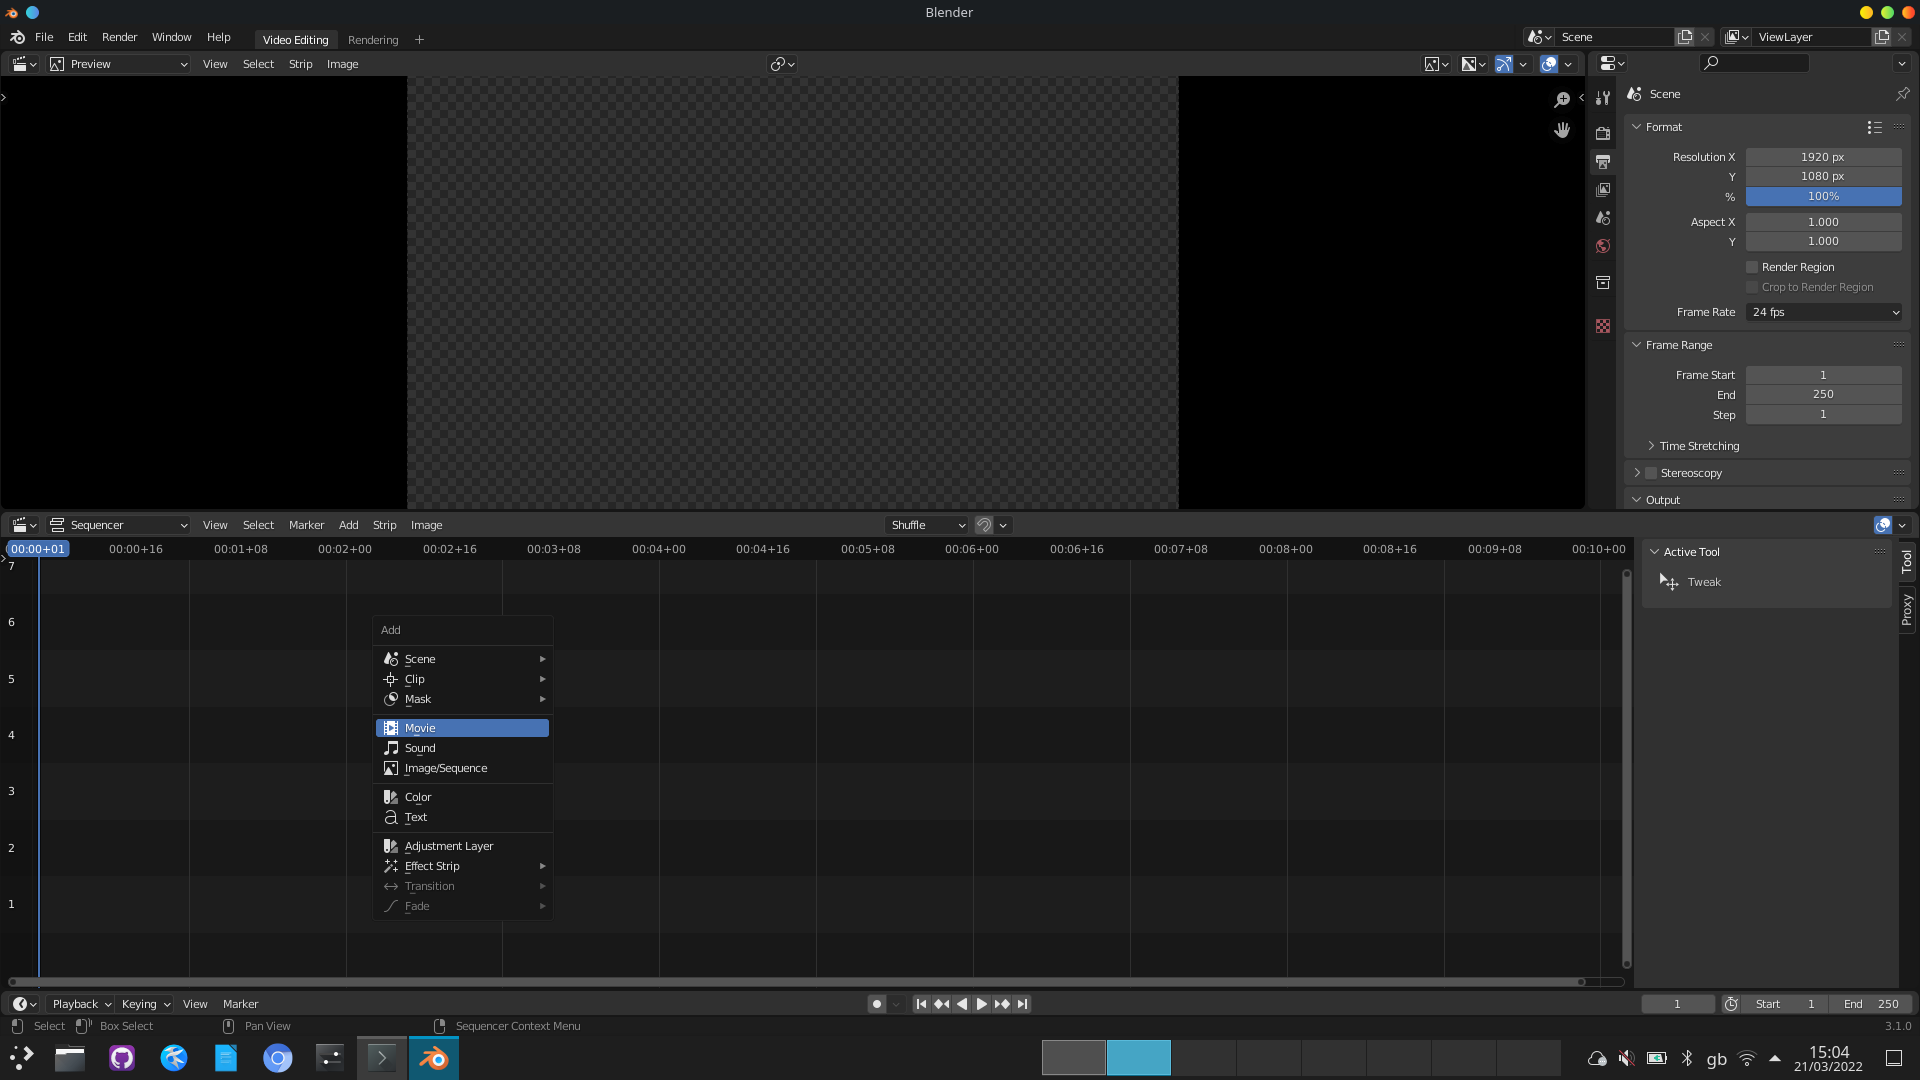
\includegraphics[width=1\linewidth]{blenderVideoEditor}
	\captionof{figure}{Blender video editor}
\end{minipage}
\begin{minipage}{.5\textwidth}
	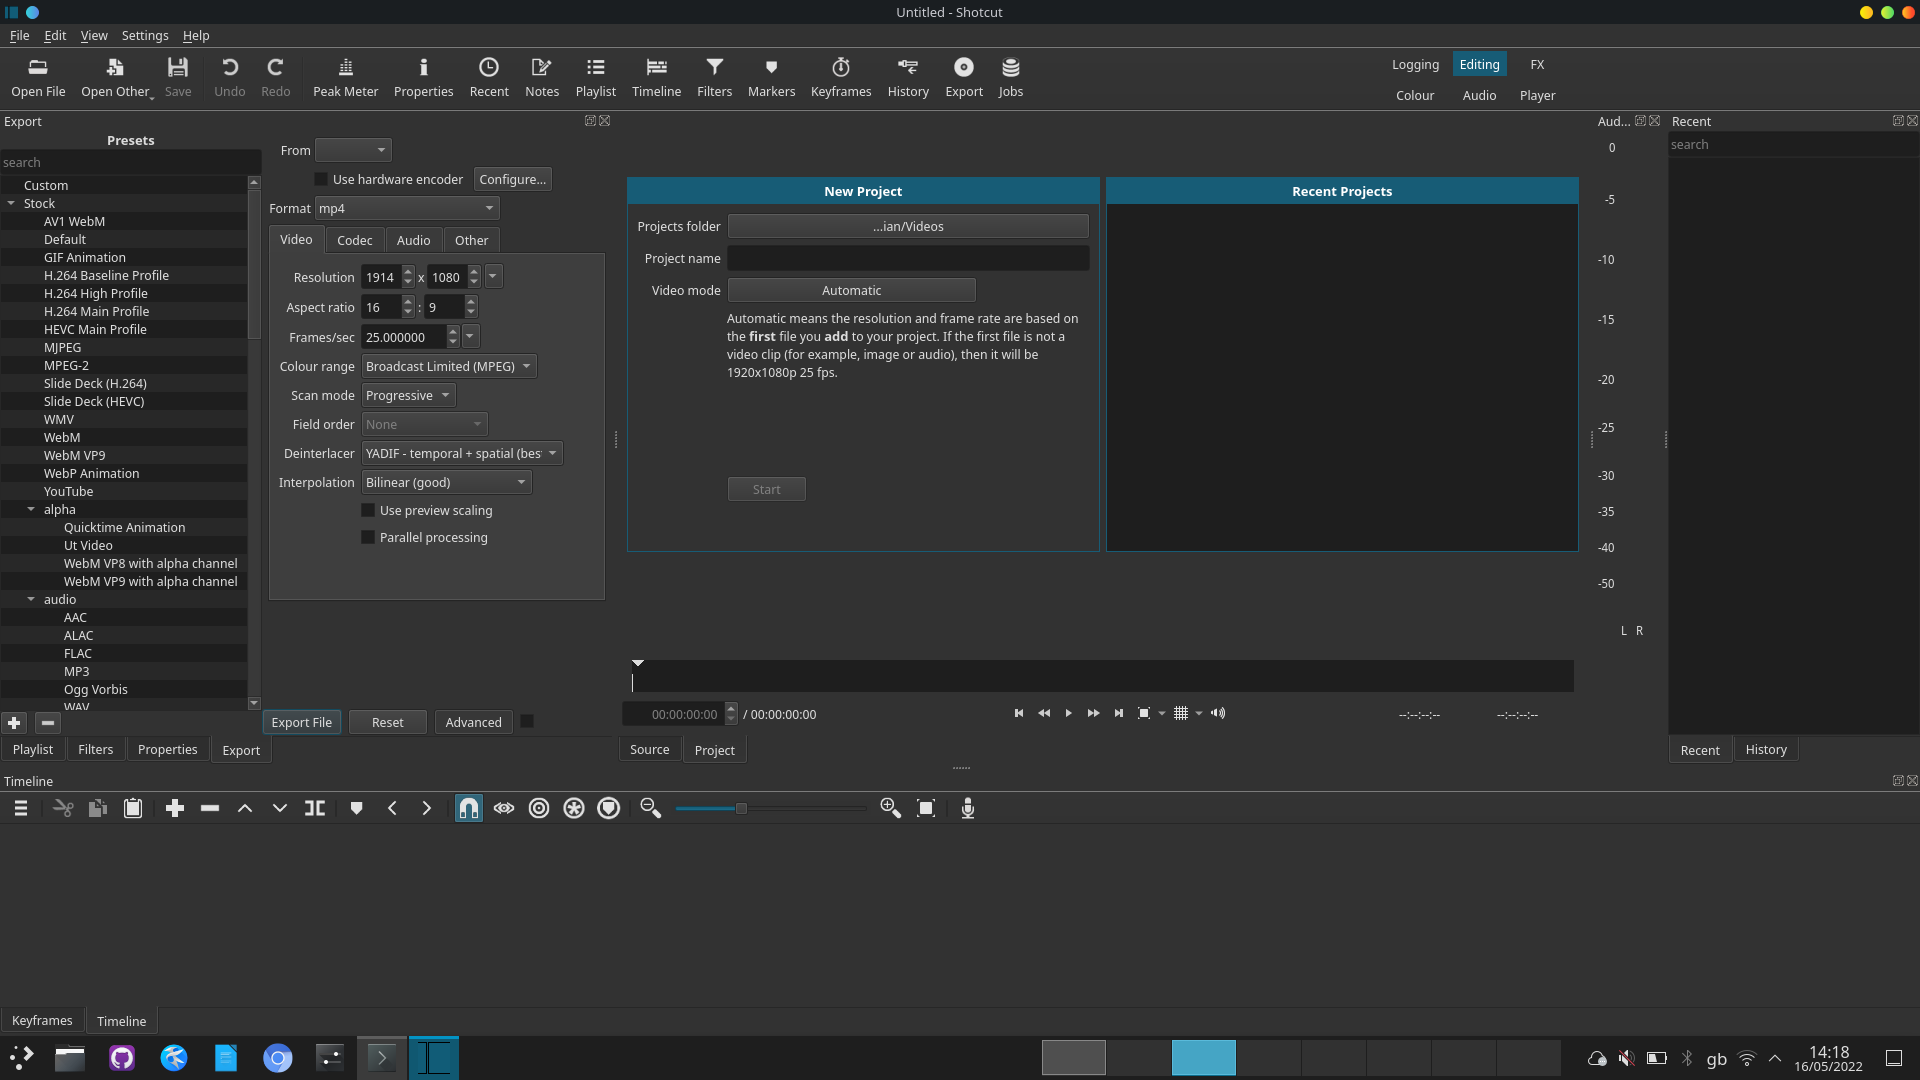
\includegraphics[width=1\linewidth]{shotcut}
	\captionof{figure}{Shotcut video editor}
\end{minipage}
\begin{minipage}{.5\textwidth}
	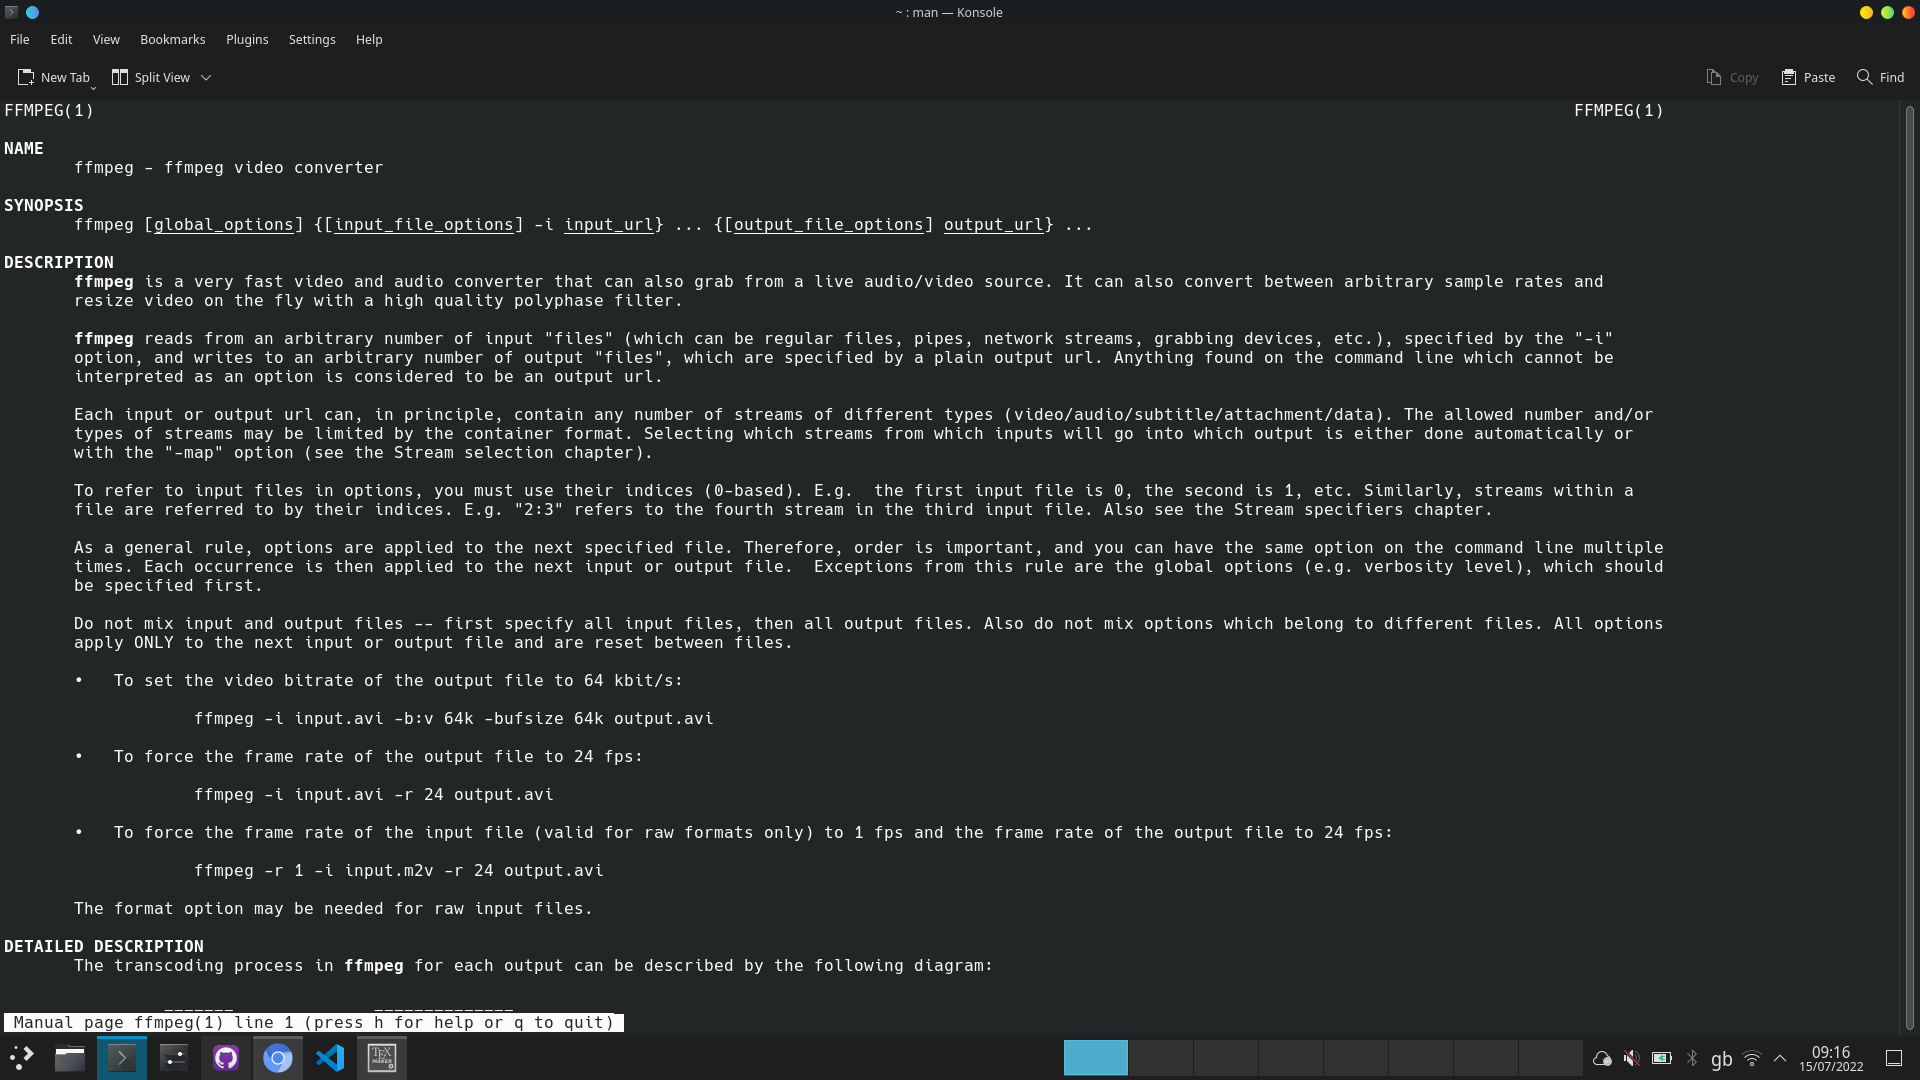
\includegraphics[width=1\linewidth]{ffmpeg}
	\captionof{figure}{FFMPEG man page}
\end{minipage}
\begin{minipage}{.5\textwidth}
	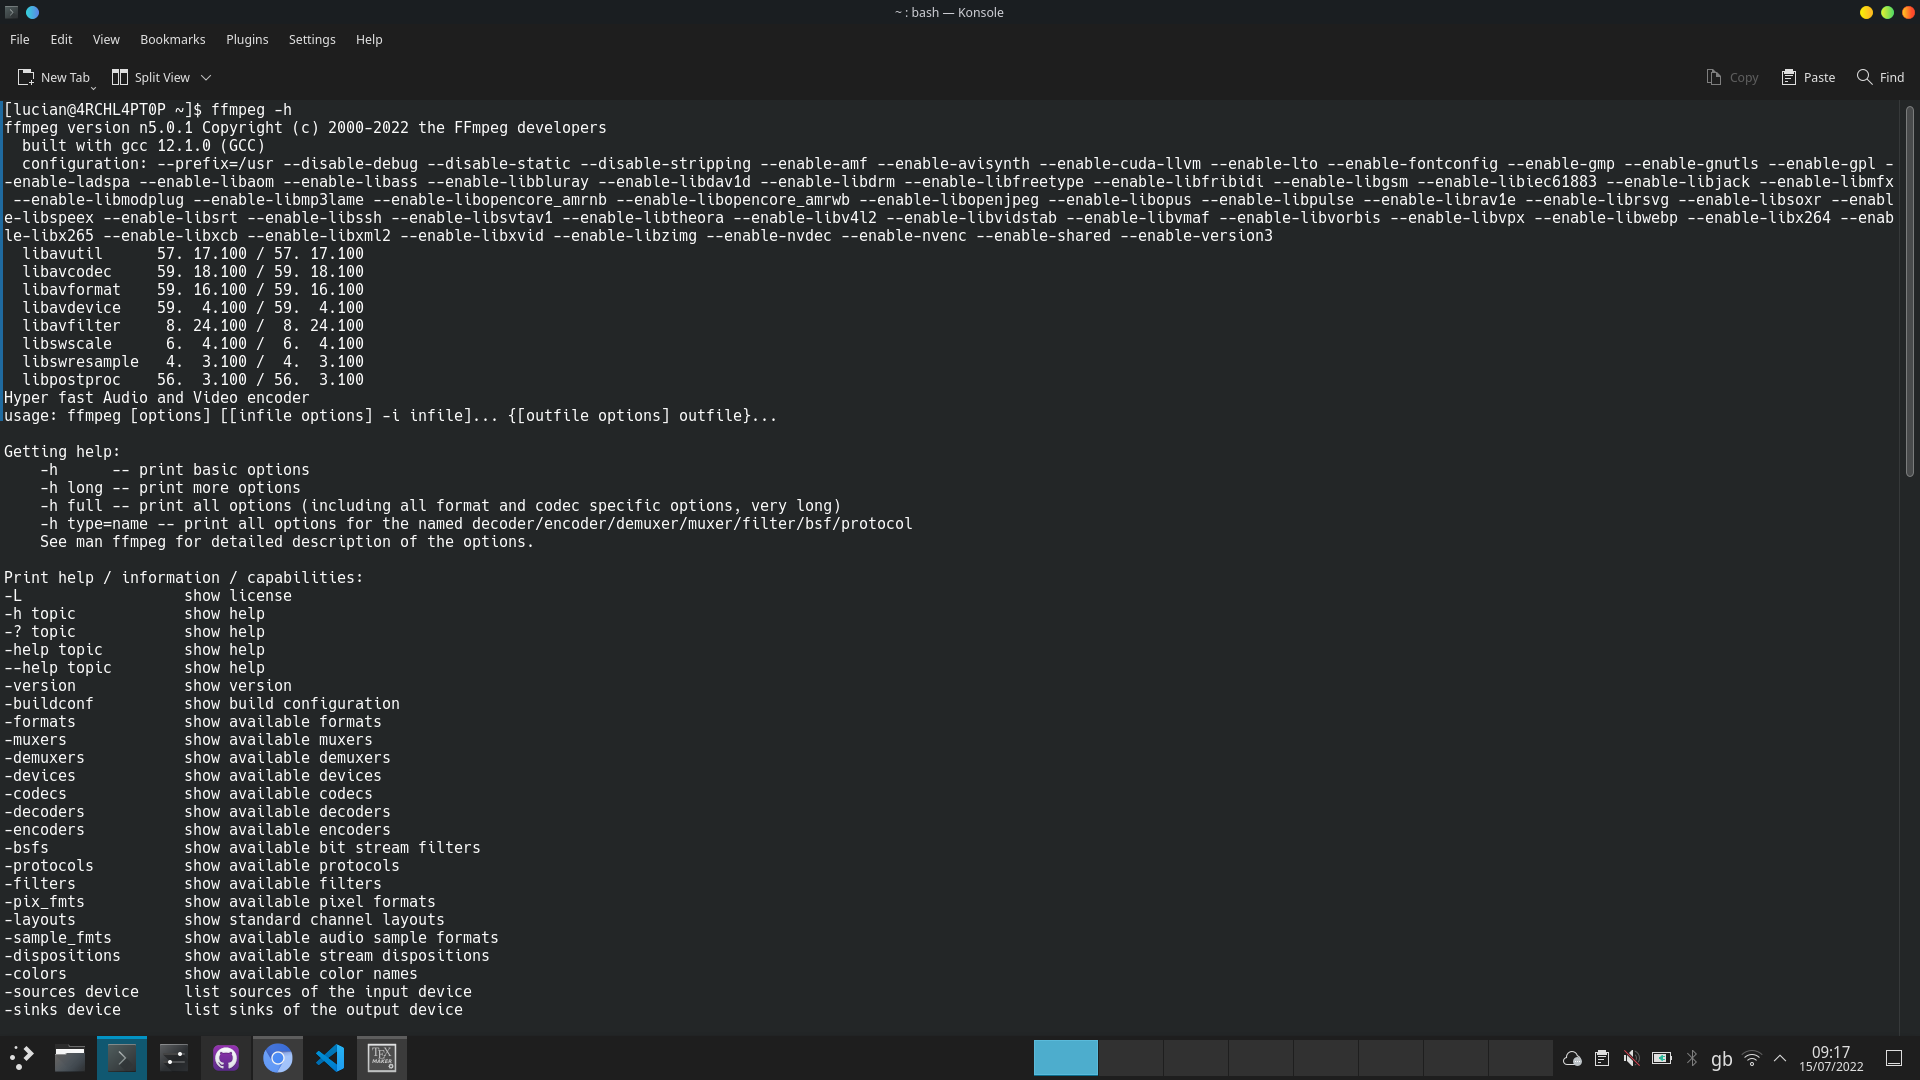
\includegraphics[width=1\linewidth]{ffmpeg2}
	\captionof{figure}{FFMPEG}
\end{minipage}
All these existing solutions do cover the main client requirement; Converting a video into a set of images. But the primary issue with them is how they are not particularly user friendly, the fact it takes too long to set up VLC to perform image extraction is the main reason the client has the need for a custom solution. These pieces of software all demonstrate the fact that simply performing the task on the most basic level required is not sufficient, it must be easy for the user to learn how to use the software and it must be a quick and simple process once they have learnt how to perform it.

\subsection{Client feedback/question}
\begin{center}
\resizebox{\textwidth}{!}{
\begin{tabular}{|p{10cm}|p{10cm}|}
\hline
Question & Client answer \\
\hline \hline
1: How will you make use of this program? & I would like to be able to use my phone and drone to use the video capture option instead of taking many still images. As the delay between pressing the button and capturing the image can cause issues. It means I could focus on flying/walking/moving smoothly and extract image later. (example photos are available)  \\
\hline
2: What exactly do you absolutely need this software to do? (what are the minimum requirements for the software to be viable?) & 
\begin{itemize}
\itemsep-0.5em 
\item Input a video 
\item select output folder 
\item select filename 
\item Program auto add a unique number i.e. castle0001 (prefix zeros essential) - Prefix could be calculated by working out number of frames from length of video 
\item Select frequency of images to be captured i.e. 1 per second or every 5 frames  
\item Choose file format i.e. jpeg, png, bmp etc  
\item Choose custom image size, source size should be default 
\item User friendly GUI – intuitive to use - Should take a new user less than a minute to figure out.
\end{itemize}
\\
\hline
3: What current software/processes do you use which will be replaced by this program? Bonus: why do you need to replace them? & Currently resort to just doing individual image on the camera.
I have used vlc video player – it is a faff, you have to use the options deep in the setting menu to auto export images. It then does it to every video you play. I have seen blender used, again, not user friendly, not quick or intuitive. I have not research blender options.  
\\
\hline
4: Which takes greater priority: ease of use vs ability to tweak final result to get optimal results? Bonus: why? & Ease of use. If its hard, it wont get used at all. \\
\hline
5: Which takes greater priority: optimising RAM usage vs optimising computational time taken? Bonus: why? & Actual processing time is not a concern, as 3d scanning is lengthy anyway. Calculating harddrive space could be useful though. I hate starting a job, then computer says half way through, not enough space. It would have taken a simple algorithm to do a quick pre check. \\
\hline
6: Are the outlined success criteria relevant (see lower section)? If not please describe additions or changes that should be made. & Yes, but reflect on above comments. \\
\hline
\end{tabular}
}
\end{center}
\begin{center}
\resizebox{\textwidth}{!}{
\begin{tabular}{|p{15cm}|}
\hline
Reasons for each question \\
\hline \hline
1: Understanding how the client will utilise the program is essential to know exactly how it should be designed and developed to meet their requirements. If i do not have a direct description of how the client plans to utilise this software, i would have to simply guess when making important decisions about the design. \\
\hline
2: Similar to the first question, i need to know what is required to produce the minimum viable product for the client. Knowing this will allow me to prioritise features. \\ 
\hline
3: Understanding why the clients existing solutions need to be replaced will help me design software which focuses on improving the areas the client had specific issues with when using other existing solutions. \\
\hline
4: Knowing this will allow me to optimise the design to the client and their required level of complexity in terms of software customisability and stuff. \\
\hline
5: This specific choice of optimisation needs to be known right from the beginning, throughout implementation decisions need to be made relating to this specific question. Since video/image data is being processed, RAM usage will likely be very high without significant optimisation. \\
\hline
6: It is very important that the success criteria i have described align with the clients own vision of how the software should work and what it should do. \\
\hline
\end{tabular}
}
\end{center}

\section{Essential features of proposed solution} \label{feat}
The absolute bare minimum requirements of the software were outlined by the client when i asked. These basic requirements are:
\begin{itemize}
\item Input a video (Take a video on disk as input, read it into memory/temp file)
\item Select output folder (User can choose where the output of the program will go)
\item Select filename (User can choose the name of the output files)
\item Program auto add a unique number i.e. castle0001, prefix zeros ESSENTIAL (Output files have number representing frame number)
\item Select frequency of images to be captured i.e. 1 per second or every 5 frames (Let user choose the rate at which frames are saved out of the input video)
\item Choose custom image size, source size should be default (User can choose to resize the output frames, by default dont resize images)
\item User friendly GUI - intuitive to use - Should take a new user less than a minute to figure out.
\end{itemize}
Other essential features which i have decided must be included based on my previous experience with photogrammetry, as well as general requirements which i think should be included even though the client has not named them specifically:
\begin{itemize}
\item Can read a variety of different formats of video files, or sets of individual images from a user-specified path on disk.
\item Can take user input to change settings.
\item Detect and remove images which are too blurry, allowing the user to define the threshold. This feature needs to be included so the user can easily clean up their dataset to improve the quality of the final result of photogrammetry.
\item Detect and remove duplicate images, allow user to define the threshold. This feature needs to be included so that duplicate data can be easily removed by the user from their dataset.
\item Detect and remove outlier images, allow user to define the threshold. This feature needs to be included so that images which will not be useful for the photogrammetry process can be removed easily.
\item Can automatically call specific open source photogrammetry software (meshroom) to start a headless photogrammetry process automatically. This should be included as it will speed up the whole meshroom photogrammetry pipeline for the user.
\item Denoise images. This is very important as input video, especially from smartphone cameras, can contain a lot of noise which could negatively affect the result of photogrammetry.
\item Minimalistic, easy to use and intuitive graphical interface. This is important as users need to be able to use the software quickly and easily, having an intuitive interface makes it possible for the user to figure out how to use the software for themselves without the need for detailed instructions.
\item Settings are grouped into ``basic'' and ``advanced'', by default advanced settings are hidden under a drop down next to the basic settings. This hides functionality that users may be unlikely to need, making it easier to navigate the program and configure the essential settings.
\end{itemize}
Some the above may need to be able to be toggled on/off by the user depending on their needs.

\section{Hardware and software requirements}
This software will require hardware with reasonable computational ability and capacity, it may be the case that reasonable CPU power and memory space is required to run the data processing on the video input. Faster hardware will result in faster processing of the videos.
Available memory could very well be a limiting factor, but determining an exact amount required is not easy as the RAM usage of the program will depend upon the size of the input data. Overall, due to the nature of video and image processing (lots of mathematical operations on a large set of data), it should be expected that a powerful computer will be required.\\\\ If possible, i will try and enable GPU acceleration of OpenCV which means that a reasonably powerful GPU may be a hardware requirement. GPU acceleration will likely be added via CUDA and not OpenCL, as i have access to reasonably powerful CUDA capable graphics cards. A CUDA supporting GPU may be a requirement.\\\\
I will try and write this software in a way which is cross-platform, so operating system wont be a major limiting factor in what devices can run the software. I will write using a compiled language, so no interpreter will need to be installed to run the software.

\section{How the problem can be solved by computational methods}
%problem is clearly defined  - able to identify current situation, end goal, possible means of reaching the end goal, and the potential obstacles
%problem needs to be computable - consider what type of calculations are required, and if these are feasible within a reasonable time frame and processing capacity
\subsection{Can the problem be solved computationally?}
My program primarily performs data processing, processing large amounts of data is a task which naturally can be performed very well on computers. The tasks outlined in section \ref{feat} can all be broken down into mathematical steps which a computer can perform. Although there may be issues with the time taken to perform these computations, as image processing is very time consuming due to the large amount of data and thus the large number of computations that need to be performed.

\subsection{Use of abstraction}
Representational abstraction can be performed to remove unnecessary details from an idea/concept. Abstraction can be used to simplify a process to make it easier to use.
My program aims to use abstraction to simplify the process of performing:
\begin{itemize}
\item Extracting frames from video input
\item Denoise extracted frames
\item Blur detection/quantification to clean the set of extracted frames
\item Comparison of image similarity to remove duplicate images from the set of extracted frames
\item Detection of ``outlier'' images which would clearly provide no benefit during the photogrammetry process
\item Running the final cleaned data through meshroom
\end{itemize}
Simplification of these processes will be done by presenting the user with abstracted controls to guide each process.\\\\
For the extraction of frames from video input, the user will be presented with options such as the number of total frames they want extracted from the video, or the desired frames to be extracted per second of video, this is an abstract control of the extraction process as the user does not need to consider the calculation of exactly how many frames to ``skip'' to get the desired amount of frames from the input.\\\\
For the denoising of extracted frames, the user will be presented with a simple control of ``denoise strength'' (or some other similar name) which allows them to choose how heavily the denoising algorithms will affect the input images without them having to be aware of any of the mathematical processes involved in denoising.\\\\
For the blur detection/quantification, the user will simply be presented with a ``blurryness'' value for each image after the calculations are complete, then they can choose a threshold to filter images out for being too blurry. This abstraction hides away many details about how exactly this ``blurryness'' value is calculated, the user is just presented with all they need to know about the process of blurry frame removal. The abstracted processes include converting the frames to grayscale, scaling down, and performing calculations such as the variation of the Laplacian filter or Fourier transforms.\\\\
For the removal of duplicate/very similar frames, the user will be presented with the option to quickly detect groups of similar images which they can then optionally automatically delete all but one of, or manually view and remove themselves.
The process of how image similarity is calculated is completely abstracted and hidden from the user, as they do not need to know about the underlying process of detecting images which may be similar.\\
Detection of ``outlier'' images will be presented to the user in a very similar way, but instead of showing them duplicate or very similar images, it will present them with frames which do not match the rest of the data at all (such as completely black frames where the camera was accidentally covered by a finger, for example).\\\\
My program will automatically call meshroom for the user if they want it to, which means that as long as they use meshroom they can use my program for their entire 3D scanning pipeline. My program will abstract the process of using meshroom to one or two simple options inside my program.

\subsection{Required input}
My program will require input data, this can be in the format of both video or sets of images. This input data is then cleaned to make it more suitable for use in photogrammetry processes. It must be validated that the input data is of the accepted formats (a variety of image and video formats, jpg, png, mp4, etc).

\subsection{Procedures and decomposition}
The core functionality of my program can very easily be broken down into smaller components, this is because the core functionality exists as a set of procedures performed as a pipeline. Each of the following can be completely isolated from one another, then brought together in a main program:
\begin{itemize}
\item Reading a video file into frames in memory or in a temp file on disk
\item Image similarity comparison
\item Outlier detection
\item Blur detection
\item Image denoising
\item Saving the final data to the users desired output location
\item Automatically calling meshroom
\end{itemize}
Each of these isolated components can then also be decomposed further to produce a detailed list of functions the program needs to function.

\subsection{Concurrence}
The main processes will take place in a pipeline, there will not be any concurrent processes aside from the user interface running and displaying information about the progress of the computation and allowing the user to cancel the process.\\\\
Running multiple parts of the pipeline at once would likely not result in any speedup as each concurrent process may take CPU/GPU time from the other(s). Additionally, implementing this concurrence would be very time consuming and complex to do in such a way that it actually provides a significant speedup.

\section{Limitations of proposed solution}
A computer with a fairly powerful processor, or (as long as I include openCV GPU acceleration) ideally a powerful GPU will be required to run more intensive functions such as image denoising in a reasonable amount of time.\\\\
The fact that video files are often heavily compressed compared to images needs to be considered. Video input simply wont produce 3D scans of equal or better quality than image input, unless professional equipment is used.\\\\
Image similarity comparison for duplicate/outlier image removal will likely be a difficult problem to solve, experimentation with various different methods will be required to find a suitable method. Unlike other functions performed inside my software, duplicate/outlier detection is not implemented in libraries such as OpenCV.

\section{Success criteria}
The core success criteria specifically defined by the client, as well as how i can measure them:
\begin{itemize}
\item Takes a video input. - Simple to test this, simply define the path to the video in the software and check to see if it loads itself properly into memory or a temp file.
\item Output location can be changed by the user. - Very simple to test this, just need to set an output path and check to see if it works.
\item Output filename can be customised by the user. - Also very simple to test this, just need to set the output filename and check to see if it works.
\item Program automatically appends frame number to the output. - Also very simple to test this, just need to run the software and check the output.
\item Frequency of frame extraction can be customised by the user by choosing either frames per second or an amount of frames to `skip' for every saved frame. - Also a simple test of running the software and verifying the input is correct.
\item User can choose to resize the output images (default no resize). - Another simple test which consists of just running the software and verifying the output images are sized correctly.
\item User friendly GUI, intuitive to use, Should take a new user less than a minute to figure out. - It is hard to quantify how user friendly and intuitive a GUI is, but the client defines that it ``should take a new user less than a minute to figure out'', so this metric will be used to measure it.
\end{itemize}
Additional success criteria specified by myself as additions or clarifications based on my interpretation of the clients feedback and initial requirements:
\begin{itemize}
\item Can reliability perform extraction of frames from an input video, and can take user input to control how many frames are extracted. Testing this is simple, send some input video, set the desired amount of output frames, run the function, and compare the output with the desired output.
\item Can quantify the ``blurryness'' of images with a reasonable degree of accuracy. This could be tested by sending a set of clear images and a set of blurry images through the algorithm and comparing the output from each, ideally frames should be classified with a 90\% accuracy.
\item Can quantify image similarity with a reasonable degree of accuracy. This could be tested by sending pairs of deliberately similar and dissimilar images and comparing how the function quantifies each pair. Exact duplicate images must be detected 100\% of the time.
\item The process of turning a video into a usable set on images is quicker than existing methods. This should be measured based on a user who is not ``used'' to any particular piece of software being used, making it a fair comparison of usability. Various different pieces of software should be tested and compared to mine in this way.
\item Can reliably remove noise from frames. This could be analysed with the use of test images, a test image can be created/sourced then a ``noisy'' version of it can be created easily. This noisy image can then be passed through the denoising algorithm then the loss from the original image can be calculated. The mean squared error algorithm (\ref{eq:3DMSE}) could be used to calculate this.
\begin{center}
\begin{equation}\label{eq:3DMSE}
MSE = \frac{1}{n} \sum_{w,h,c}(y_{w,h,c}-\hat{y}_{w,h,c})^2
\end{equation}
\begin{conditions}
 n & number of data points\\
 y & expected values\\
 \hat{y} & output values\\
 w & represents image width\\
 h & represents image height\\
 c & represents image channels
\end{conditions}
\end{center}
\item The process of extracting frames from videos is faster than using other software. The comparison of speed should also take into account different processing being performed, for example, most video editing software can extract frames from video but not all may be capable of denoising the images. Speed comparisons should be done only when the same output is being produced, making the comparison fair.
\end{itemize}


\chapter{Design}
\thispagestyle{fancy}



\end{document}